\begin{minipage}[t]{170mm}
\vspace{3mm}
\section*{Ikke-kommutativ studenterrådgivning}
\emph{Kære brevkasse}

\emph{Hvorfor er  lilla den farve jeg synes bedst om?}

\emph{Hilsen, en husalf}

\subsection*{Svar}
Dette faktum kan med lethed forklares. Campens mandlige ko er flere gange blevet observeret i en lilla t-shirt, som reklamerer for et konkurrerende arrangement. Kombinationen af den grimme og meget umandlige farve og tøjets forræderiske påtryk, udløser i dig et håb om, at han vil kaste det fra sig, og du vil kunne opfange t-shirten som gave. Du tror så, at dette vil medføre din frigivelse, men dette er heldigvis ikke sandt, da vasaller ikke har ejerskabet, men kun brugsretten over marker og alfe, og han derfor ikke er den rette til at skære dit bånd.

Så kaffe vil laves, når kaffe skal til.

{\flushright\emph{Hilsen den ikke-kommutative studenterrådgivning}}
\vspace{3mm}
\section*{Dagens opgave}

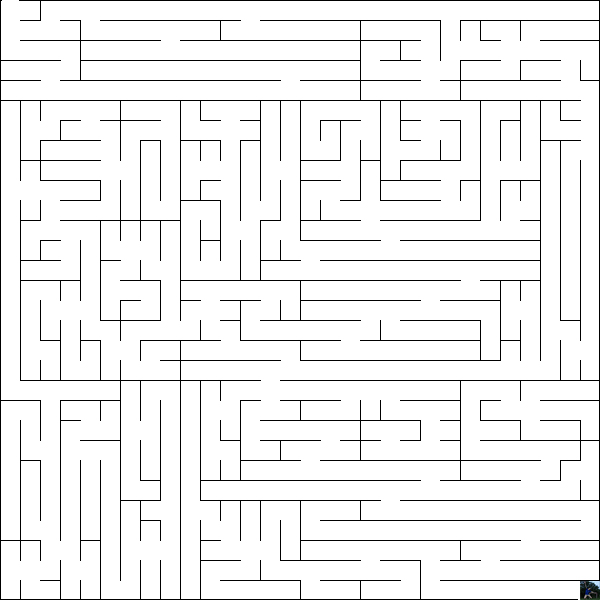
\includegraphics[width=\textwidth]{mazemedfynbo.jpg}


\end{minipage}
